% Editable textbook TikZ, initially imported from the verified semantic plate.
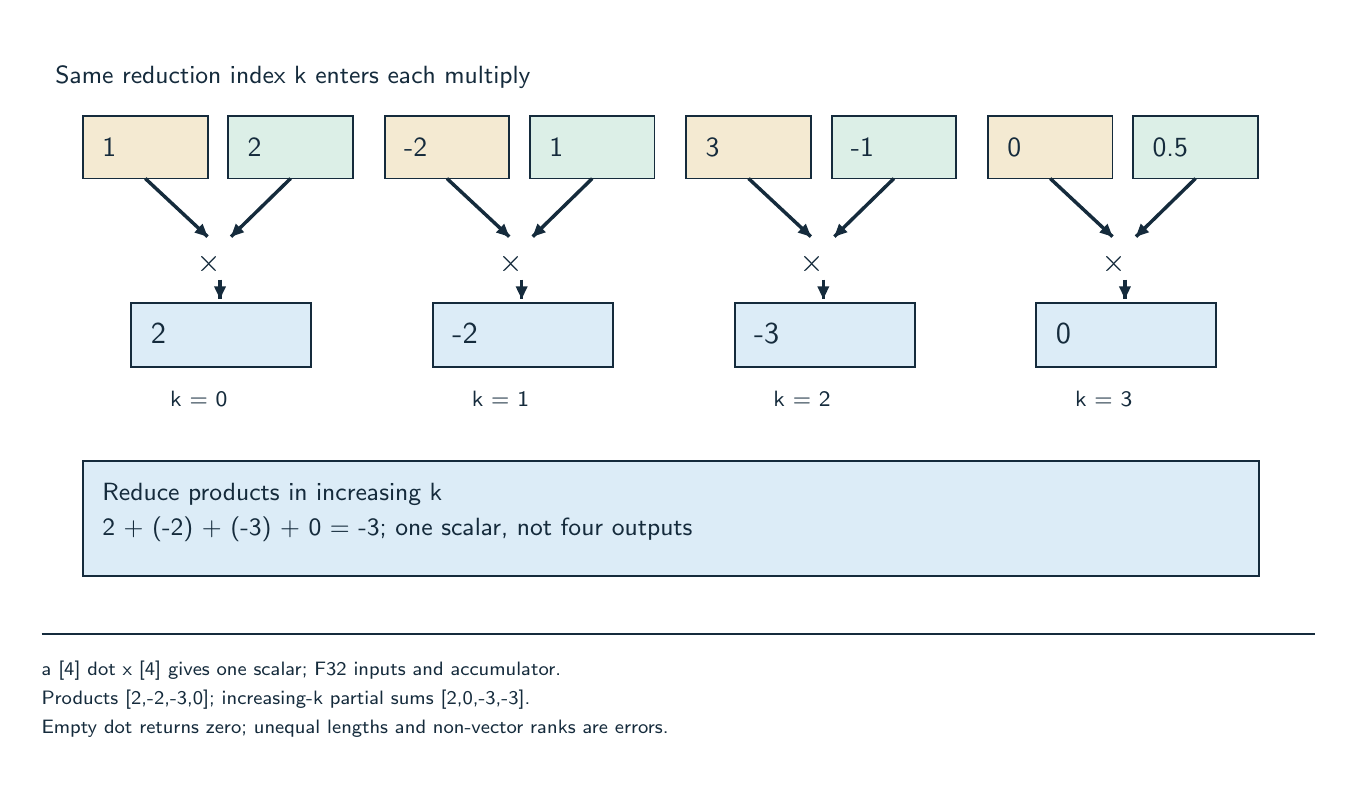
\begin{tikzpicture}[x=.5pt,y=-.5pt]
\path[use as bounding box] (30,170) rectangle (975,700);
\node[inner sep=0pt,outer sep=0pt,anchor=base west,text={rgb,255:red,21;green,43;blue,60},font=\sffamily\fontsize{9.5}{11.4}\selectfont] at (50,210) {Same reduction index k enters each multiply};
\path[fill={rgb,255:red,244;green,234;blue,210},draw={rgb,255:red,21;green,43;blue,60},line width=0.7pt] (70.0,234.0) rectangle (160.0,279.0);
\node[inner sep=0pt,outer sep=0pt,anchor=base west,text={rgb,255:red,21;green,43;blue,60},font=\sffamily\fontsize{10.0}{12.0}\selectfont] at (84,263) {1};
\path[fill={rgb,255:red,220;green,239;blue,231},draw={rgb,255:red,21;green,43;blue,60},line width=0.7pt] (175.0,234.0) rectangle (265.0,279.0);
\node[inner sep=0pt,outer sep=0pt,anchor=base west,text={rgb,255:red,21;green,43;blue,60},font=\sffamily\fontsize{10.0}{12.0}\selectfont] at (189,263) {2};
\draw[fill=none,draw={rgb,255:red,21;green,43;blue,60},line width=1.25pt] (115,279) -- (160,321);
\path[fill={rgb,255:red,21;green,43;blue,60},draw=none,line width=0.5pt] (160.00,321.00) -- (150.45,318.04) -- (156.39,311.68) -- cycle;
\draw[fill=none,draw={rgb,255:red,21;green,43;blue,60},line width=1.25pt] (220,279) -- (177,321);
\path[fill={rgb,255:red,21;green,43;blue,60},draw=none,line width=0.5pt] (177.00,321.00) -- (180.40,311.60) -- (186.48,317.82) -- cycle;
\node[inner sep=0pt,outer sep=0pt,anchor=base west,text={rgb,255:red,21;green,43;blue,60},font=\sffamily\fontsize{12.0}{14.399999999999999}\selectfont] at (152,347) {×};
\draw[fill=none,draw={rgb,255:red,21;green,43;blue,60},line width=1.25pt] (169,352) -- (169,366);
\path[fill={rgb,255:red,21;green,43;blue,60},draw=none,line width=0.5pt] (169.00,366.00) -- (164.65,357.00) -- (173.35,357.00) -- cycle;
\path[fill={rgb,255:red,220;green,236;blue,247},draw={rgb,255:red,21;green,43;blue,60},line width=0.7pt] (105.0,369.0) rectangle (235.0,415.0);
\node[inner sep=0pt,outer sep=0pt,anchor=base west,text={rgb,255:red,21;green,43;blue,60},font=\sffamily\fontsize{10.5}{12.6}\selectfont] at (119,398) {2};
\node[inner sep=0pt,outer sep=0pt,anchor=base west,text={rgb,255:red,21;green,43;blue,60},font=\sffamily\fontsize{8.5}{10.2}\selectfont] at (133,444) {k = 0};
\path[fill={rgb,255:red,244;green,234;blue,210},draw={rgb,255:red,21;green,43;blue,60},line width=0.7pt] (288.0,234.0) rectangle (378.0,279.0);
\node[inner sep=0pt,outer sep=0pt,anchor=base west,text={rgb,255:red,21;green,43;blue,60},font=\sffamily\fontsize{10.0}{12.0}\selectfont] at (302,263) {-2};
\path[fill={rgb,255:red,220;green,239;blue,231},draw={rgb,255:red,21;green,43;blue,60},line width=0.7pt] (393.0,234.0) rectangle (483.0,279.0);
\node[inner sep=0pt,outer sep=0pt,anchor=base west,text={rgb,255:red,21;green,43;blue,60},font=\sffamily\fontsize{10.0}{12.0}\selectfont] at (407,263) {1};
\draw[fill=none,draw={rgb,255:red,21;green,43;blue,60},line width=1.25pt] (333,279) -- (378,321);
\path[fill={rgb,255:red,21;green,43;blue,60},draw=none,line width=0.5pt] (378.00,321.00) -- (368.45,318.04) -- (374.39,311.68) -- cycle;
\draw[fill=none,draw={rgb,255:red,21;green,43;blue,60},line width=1.25pt] (438,279) -- (395,321);
\path[fill={rgb,255:red,21;green,43;blue,60},draw=none,line width=0.5pt] (395.00,321.00) -- (398.40,311.60) -- (404.48,317.82) -- cycle;
\node[inner sep=0pt,outer sep=0pt,anchor=base west,text={rgb,255:red,21;green,43;blue,60},font=\sffamily\fontsize{12.0}{14.399999999999999}\selectfont] at (370,347) {×};
\draw[fill=none,draw={rgb,255:red,21;green,43;blue,60},line width=1.25pt] (387,352) -- (387,366);
\path[fill={rgb,255:red,21;green,43;blue,60},draw=none,line width=0.5pt] (387.00,366.00) -- (382.65,357.00) -- (391.35,357.00) -- cycle;
\path[fill={rgb,255:red,220;green,236;blue,247},draw={rgb,255:red,21;green,43;blue,60},line width=0.7pt] (323.0,369.0) rectangle (453.0,415.0);
\node[inner sep=0pt,outer sep=0pt,anchor=base west,text={rgb,255:red,21;green,43;blue,60},font=\sffamily\fontsize{10.5}{12.6}\selectfont] at (337,398) {-2};
\node[inner sep=0pt,outer sep=0pt,anchor=base west,text={rgb,255:red,21;green,43;blue,60},font=\sffamily\fontsize{8.5}{10.2}\selectfont] at (351,444) {k = 1};
\path[fill={rgb,255:red,244;green,234;blue,210},draw={rgb,255:red,21;green,43;blue,60},line width=0.7pt] (506.0,234.0) rectangle (596.0,279.0);
\node[inner sep=0pt,outer sep=0pt,anchor=base west,text={rgb,255:red,21;green,43;blue,60},font=\sffamily\fontsize{10.0}{12.0}\selectfont] at (520,263) {3};
\path[fill={rgb,255:red,220;green,239;blue,231},draw={rgb,255:red,21;green,43;blue,60},line width=0.7pt] (611.0,234.0) rectangle (701.0,279.0);
\node[inner sep=0pt,outer sep=0pt,anchor=base west,text={rgb,255:red,21;green,43;blue,60},font=\sffamily\fontsize{10.0}{12.0}\selectfont] at (625,263) {-1};
\draw[fill=none,draw={rgb,255:red,21;green,43;blue,60},line width=1.25pt] (551,279) -- (596,321);
\path[fill={rgb,255:red,21;green,43;blue,60},draw=none,line width=0.5pt] (596.00,321.00) -- (586.45,318.04) -- (592.39,311.68) -- cycle;
\draw[fill=none,draw={rgb,255:red,21;green,43;blue,60},line width=1.25pt] (656,279) -- (613,321);
\path[fill={rgb,255:red,21;green,43;blue,60},draw=none,line width=0.5pt] (613.00,321.00) -- (616.40,311.60) -- (622.48,317.82) -- cycle;
\node[inner sep=0pt,outer sep=0pt,anchor=base west,text={rgb,255:red,21;green,43;blue,60},font=\sffamily\fontsize{12.0}{14.399999999999999}\selectfont] at (588,347) {×};
\draw[fill=none,draw={rgb,255:red,21;green,43;blue,60},line width=1.25pt] (605,352) -- (605,366);
\path[fill={rgb,255:red,21;green,43;blue,60},draw=none,line width=0.5pt] (605.00,366.00) -- (600.65,357.00) -- (609.35,357.00) -- cycle;
\path[fill={rgb,255:red,220;green,236;blue,247},draw={rgb,255:red,21;green,43;blue,60},line width=0.7pt] (541.0,369.0) rectangle (671.0,415.0);
\node[inner sep=0pt,outer sep=0pt,anchor=base west,text={rgb,255:red,21;green,43;blue,60},font=\sffamily\fontsize{10.5}{12.6}\selectfont] at (555,398) {-3};
\node[inner sep=0pt,outer sep=0pt,anchor=base west,text={rgb,255:red,21;green,43;blue,60},font=\sffamily\fontsize{8.5}{10.2}\selectfont] at (569,444) {k = 2};
\path[fill={rgb,255:red,244;green,234;blue,210},draw={rgb,255:red,21;green,43;blue,60},line width=0.7pt] (724.0,234.0) rectangle (814.0,279.0);
\node[inner sep=0pt,outer sep=0pt,anchor=base west,text={rgb,255:red,21;green,43;blue,60},font=\sffamily\fontsize{10.0}{12.0}\selectfont] at (738,263) {0};
\path[fill={rgb,255:red,220;green,239;blue,231},draw={rgb,255:red,21;green,43;blue,60},line width=0.7pt] (829.0,234.0) rectangle (919.0,279.0);
\node[inner sep=0pt,outer sep=0pt,anchor=base west,text={rgb,255:red,21;green,43;blue,60},font=\sffamily\fontsize{10.0}{12.0}\selectfont] at (843,263) {0.5};
\draw[fill=none,draw={rgb,255:red,21;green,43;blue,60},line width=1.25pt] (769,279) -- (814,321);
\path[fill={rgb,255:red,21;green,43;blue,60},draw=none,line width=0.5pt] (814.00,321.00) -- (804.45,318.04) -- (810.39,311.68) -- cycle;
\draw[fill=none,draw={rgb,255:red,21;green,43;blue,60},line width=1.25pt] (874,279) -- (831,321);
\path[fill={rgb,255:red,21;green,43;blue,60},draw=none,line width=0.5pt] (831.00,321.00) -- (834.40,311.60) -- (840.48,317.82) -- cycle;
\node[inner sep=0pt,outer sep=0pt,anchor=base west,text={rgb,255:red,21;green,43;blue,60},font=\sffamily\fontsize{12.0}{14.399999999999999}\selectfont] at (806,347) {×};
\draw[fill=none,draw={rgb,255:red,21;green,43;blue,60},line width=1.25pt] (823,352) -- (823,366);
\path[fill={rgb,255:red,21;green,43;blue,60},draw=none,line width=0.5pt] (823.00,366.00) -- (818.65,357.00) -- (827.35,357.00) -- cycle;
\path[fill={rgb,255:red,220;green,236;blue,247},draw={rgb,255:red,21;green,43;blue,60},line width=0.7pt] (759.0,369.0) rectangle (889.0,415.0);
\node[inner sep=0pt,outer sep=0pt,anchor=base west,text={rgb,255:red,21;green,43;blue,60},font=\sffamily\fontsize{10.5}{12.6}\selectfont] at (773,398) {0};
\node[inner sep=0pt,outer sep=0pt,anchor=base west,text={rgb,255:red,21;green,43;blue,60},font=\sffamily\fontsize{8.5}{10.2}\selectfont] at (787,444) {k = 3};
\path[fill={rgb,255:red,220;green,236;blue,247},draw={rgb,255:red,21;green,43;blue,60},line width=0.7pt] (70.0,483.0) rectangle (920.0,566.0);
\node[inner sep=0pt,outer sep=0pt,anchor=base west,text={rgb,255:red,21;green,43;blue,60},font=\sffamily\fontsize{9.0}{10.799999999999999}\selectfont] at (84,512) {Reduce products in increasing k};
\node[inner sep=0pt,outer sep=0pt,anchor=base west,text={rgb,255:red,21;green,43;blue,60},font=\sffamily\fontsize{9.0}{10.799999999999999}\selectfont] at (84,537) {2 + (-2) + (-3) + 0 = -3; one scalar, not four outputs};
\draw[fill=none,draw={rgb,255:red,21;green,43;blue,60},line width=0.75pt] (40,608) -- (960,608);
\node[inner sep=0pt,outer sep=0pt,anchor=base west,text={rgb,255:red,21;green,43;blue,60},font=\sffamily\fontsize{7.5}{9.0}\selectfont] at (40,638) {a [4] dot x [4] gives one scalar; F32 inputs and accumulator.};
\node[inner sep=0pt,outer sep=0pt,anchor=base west,text={rgb,255:red,21;green,43;blue,60},font=\sffamily\fontsize{7.5}{9.0}\selectfont] at (40,659) {Products [2,-2,-3,0]; increasing-k partial sums [2,0,-3,-3].};
\node[inner sep=0pt,outer sep=0pt,anchor=base west,text={rgb,255:red,21;green,43;blue,60},font=\sffamily\fontsize{7.5}{9.0}\selectfont] at (40,680) {Empty dot returns zero; unequal lengths and non-vector ranks are errors.};
\end{tikzpicture}
